
% Include LaTeX packages
\documentclass[conference]{styles/acmsiggraph}
\usepackage{comment} % enables the use of multi-line comments (\ifx \fi)
\usepackage{fullpage}
\usepackage{enumitem}
\usepackage{amsmath,amsthm,amssymb}
\usepackage{listings}
\usepackage{graphicx}
\usepackage{etoolbox}
\usepackage{verbatim}
\usepackage{minted}
\usepackage[dvipsnames]{xcolor}
\usepackage{fancyvrb}
\usepackage{hyperref}
\usepackage{menukeys}
\usepackage{titlesec}
\usepackage{csquotes}
\usepackage{placeins}
\usepackage{caption}
\usepackage{subcaption}
\usepackage{algorithm} 
\usepackage{booktabs}
\usepackage{cases} 
\usepackage{algpseudocode}
\usepackage{unicode-math}
\newcommand{\?}{\stackrel{?}{=}}
\renewcommand\qedsymbol{$\blacksquare$}
\usepackage{tikz}

\usepackage[T1]{fontenc}
\usepackage{kantlipsum}
\usepackage[usenames,dvipsnames]{xcolor}
\usepackage[breakable, theorems, skins]{tcolorbox}
\tcbset{enhanced}

\DeclareRobustCommand{\myalignbox}[2][gray!20]{%
\begin{tcolorbox}[   %% Adjust the following parameters at will.
        breakable,
        left=0pt,
        right=0pt,
        top=0pt,
        bottom=12pt,
        colback=#1,
        colframe=#1,
        width=\dimexpr\textwidth\relax, 
        enlarge left by=0mm,
        boxsep=5pt,
        arc=0pt,outer arc=0pt,
        ]
        #2
\end{tcolorbox}
}

\DeclareRobustCommand{\myTIKZbox}[2][gray!20]{%
\begin{tcolorbox}[   %% Adjust the following parameters at will.
        breakable,
        left=0pt,
        right=0pt,
        top=10pt,
        bottom=12pt,
        colback=#1,
        colframe=#1,
        width=\dimexpr\textwidth\relax, 
        enlarge left by=0mm,
        boxsep=5pt,
        arc=0pt,outer arc=0pt,
        ]
        #2
\end{tcolorbox}
}

\DeclareRobustCommand{\mybox}[2][gray!20]{%
\begin{tcolorbox}[   %% Adjust the following parameters at will.
        breakable,
        left=0pt,
        right=0pt,
        top=0pt,
        bottom=0pt,
        colback=#1,
        colframe=#1,
        width=\dimexpr\textwidth\relax, 
        enlarge left by=0mm,
        boxsep=5pt,
        arc=0pt,outer arc=0pt,
        ]
        #2
\end{tcolorbox}
}

% Set additional LaTeX options
\setlength{\parskip}{.8mm}
\setcounter{MaxMatrixCols}{20}
\hypersetup{
	colorlinks=true,
	urlcolor=[rgb]{0.97,0,0.30},
	anchorcolor={0.97,0,0.30},
	linkcolor=black,
	filecolor=[rgb]{0.97,0,0.30},
}

% Define title, author, and affiliation information
\title{\huge PSET 6 \\ \LARGE {CS124: Data Structures and Algorithms \\ Prof. Mitzenmacher}}
\author{\Large Dhilan Ramaprasad \\ dhilanramaprasad@college.harvard.edu}
\pdfauthor{Student Name}

% Redefine \VerbatimInput
\RecustomVerbatimCommand{\VerbatimInput}{VerbatimInput}%
{fontsize=\footnotesize,
 %
 frame=lines, % top and bottom rule only
 framesep=2em, % separation between frame and text
 rulecolor=\color{Gray},
 %
 label=\fbox{\color{Black}\textbf{OUTPUT}},
 labelposition=topline,
 %
 commandchars=\|\(\), % escape character and argument delimiters for commands within the verbatim
 commentchar=* % comment character
}

% Set addditional formatting options
\titlespacing*{\section}{0pt}{5.5ex plus 1ex minus .2ex}{2ex}
\titlespacing*{\subsection}{0pt}{3ex}{2ex}
\setcounter{secnumdepth}{4}
\renewcommand\theparagraph{\thesubsubsection.\arabic{paragraph}}
\newcommand\subsubsubsection{\paragraph}

% Define a convenient norm symbol
\newcommand{\norm}[1]{\left\lVert#1\right\rVert}
\renewcommand{\vec}[1]{\mathbf{#1}}

% Define a macro for hiding answers
\newbool{hideanswers} \setbool{hideanswers}{false}
\newenvironment{answer}{}{}
\ifbool{hideanswers}{\AtBeginEnvironment{answer}{\comment} %
\AtEndEnvironment{answer}{\endcomment}}{}

% Define text formatting for points and normals
\newcommand{\points}[1]{\hfill \normalfont{(\textit{#1pts})}}
\newcommand{\pointsin}[1]{\normalfont{(\textit{#1pts})}}







%%%%%%%%%%%%%%%%%%%%%%%%%%%%%%%%%%%%%%%
%%%%%%%%%%%%%%%%%%%%%%%%%%%%%%%%%%%%%%%
%%%%%%%%%%%%%%%%%%%%%%%%%%%%%%%%%%%%%%%
%%%%%%%%%%%%%%%%%%%%%%%%%%%%%%%%%%%%%%%
%%%%%%%%%%%%%%%%%%%%%%%%%%%%%%%%%%%%%%%

         %  START HERE  %

%%%%%%%%%%%%%%%%%%%%%%%%%%%%%%%%%%%%%%%
%%%%%%%%%%%%%%%%%%%%%%%%%%%%%%%%%%%%%%%
%%%%%%%%%%%%%%%%%%%%%%%%%%%%%%%%%%%%%%%
%%%%%%%%%%%%%%%%%%%%%%%%%%%%%%%%%%%%%%%
%%%%%%%%%%%%%%%%%%%%%%%%%%%%%%%%%%%%%%%

\begin{document}
\maketitle

\textbf{Collaborator}: No one :( \\
\textbf{Others:} A little advice from Ryan G. \\
\\ \\
I \textbf{\textit{still}} haven't been to Esther/Amy's office hours in a long time.  I miss going to their office hours :( \\
I \textbf{\textit{still}} haven't been to Rachel/Rose's section in a long time.  I miss going to their section :( \\

Now, I, uh, really, uh, like, miss Professor Mitzenmacher :( \\

I \textbf{\textit{still}} don't miss Piazza.

\newpage


\section{Partially Reflecting Boundary---Random Walk}
%%%%%%%%%%%%%%%%%%
%   Question #1  %
%%%%%%%%%%%%%%%%%%

\begin{figure}[h!]
    \centering
    \includegraphics[width=0.8\textwidth]{Q1.png}
    \caption{Probabilistic Model of Random Walk}
    \label{fig:Q1Model}
\end{figure}
\FloatBarrier

Given a partially reflecting boundary at $0$, we can model our probabilistic model of step-advancement (\enquote{moves}) as in Figure \ref{fig:Q1Model} above.

Now, let $S$ represent the number of remaining steps (or moves) to reach $n$.  We can take:

\myalignbox{
\begin{align}
    S_N &= 0\\
    S_i &= \frac{1}{2}S_{i-1} + \frac{1}{2}S_{i+1} + 1 & \text{for } 1 \leq i \leq n-1
\end{align}}

Our base case for $i=0$ is worth noting, too:

\myalignbox{
\begin{align}
    S_0 &= \frac{1}{2}S_{1} + \frac{1}{2}S_{0} + 1 = 2 \left(\frac{1}{2}S_1 + 1 \right) = S_1 + 2 \label{eq:E0}
\end{align}}

A first look at a graphical interpretation for various values of $n$ indicates a concave-down quadratic function (unrolling method shown in detail below when solving for constants) which we can represent as the general factored form with constants $a$, $s$, and $r$:
$$ E_i = -a(i-s)(i-r) $$

Of course, given our base case where $E_n \eqiv 0$, we can rewrite our expected form: 
$$ E_i = -a(i-\mathbf{n})(i-r) $$

Now our goal is to find $a$ and $r$.  Performing a similar analysis as to that done in Section 8, we can unwrap some terms:
\begin{align}
    E_n &= 0\\
    E_{n-1} &= \frac{1}{2} E_{n-2} + 1 = -a(n-1-n)(n-1-r) = a(n-1-r) \label{eq:Expectation of N-1}\\
    E_{n-2} &= \frac{1}{2} E_{n-3} + \frac{1}{2} E_{n-1} + 1 = -a(n-2-n)(n-2-r) = 2a(n-2-r)
\end{align}

We can perform a back-substitution now that we know the value of $E_{n-2}$ which is required to evaluate the left hand side of Equation \ref{eq:Expectation of N-1}:
\begin{align*}
    \frac{1}{2} \left(2a(n-2-r)\right) + 1 &= a(n-1-r)\\
    1 &= a
\end{align*}

And we find a further reduced expected form:
\begin{equation}
    E_i = -1(i-n)(x-r) \label{EQ:genForm1}
\end{equation}


A method to solve for $r$ was not immediately clear to me, so I returned to experimentation.  Given $n=3$, I could create a set of expected coordinates (as I did above to predict the concave-down quadratic function):

\begin{align}
    n &= 3\\
    E_3 &= 0\\
    E_0 &= E_1 + 2 & \text{from Equation \ref{eq:E0}}\\
    E_1 &= \frac{1}{2}E_0 + \frac{1}{2}E_2 + 1 \implies E_2 +4 & \text{implied via substitution}\\
    E_2 &= \frac{1}{2}E_1 + \frac{1}{2}E_3 + 1 \implies 6
\end{align}

Back-substitution, again, yields a full set of coordinates:
$$(3,0),\ (2,6),\ (1, 10),\ (0,12)$$

Using our most up-to-date general form (Equation \ref{EQ:genForm1}), we can determine $r$ for the specific case of $n = 3$:
\begin{align*}
    E_2 = -(2-3)(2-r) = 6\\
    r = -4\\
    \text{Guess: } r = -n - 1
\end{align*}

With our guess of $r = -n-1$, we can re-write our final generalized form for expected remaining steps given $n$ and current position, $i$:
\myalignbox{\begin{align}
    E_i &= -(i-n)(i-(-n-1)) \\
    E_i &= -(i-n)(i+n+1)
\end{align}}

By unrolling with different values for $n$, it can be confirmed that this general solution to the recurrence is correct.

\newpage


\section{MAX FLOW = MIN CUT}
%%%%%%%%%%%%%%%%%%
%   Question #2  %
%%%%%%%%%%%%%%%%%%

\textit{I apologize for not drawing this out in Tikz---time constraints led me to stick to handwritten graphics.}

Using the \textbf{Ford-Fulkerson} algorithm, I performed the method of augmenting paths on the given graph:
\begin{figure}[h!]
    \centering
    \includegraphics[width=0.6\textwidth]{P2 Figs/2.0.PNG}
    \caption{Original Graph}
    \label{fig:2.0}
\end{figure}
\FloatBarrier

Residual graphs during Ford-Fulkerson and component depth-first search:
\begin{figure}[h!]
    \centering
    \begin{subfigure}[b]{0.4\columnwidth}
        \includegraphics[width=.92\linewidth]{P2 Figs/2.1.PNG}
        \caption{S-A-B-T}
        \label{fig:2.1}
    \end{subfigure}
    \begin{subfigure}[b]{0.4\columnwidth}
        \includegraphics[width=.92\linewidth]{P2 Figs/2.2.PNG}
        \caption{S-A-E-T}
        \label{fig:2.2}
    \end{subfigure}
    \begin{subfigure}[b]{0.4\columnwidth}
        \includegraphics[width=.92\linewidth]{P2 Figs/2.3.PNG}
        \caption{S-C-A-D-T}
        \label{fig:2.3}
    \end{subfigure}
    \begin{subfigure}[b]{0.4\columnwidth}
        \includegraphics[width=.92\linewidth]{P2 Figs/2.4.PNG}
        \caption{S-C-D-T}
        \label{fig:2.4}
    \end{subfigure}
    \begin{subfigure}[b]{0.4\columnwidth}
        \includegraphics[width=.92\linewidth]{P2 Figs/2.5.PNG}
        \caption{S-C-E-T}
        \label{fig:2.5}
    \end{subfigure}
\end{figure}
\FloatBarrier

By the step shown in Figure \ref{fig:2.5}, we see no more paths from $s$ to $t$, so the Ford-Fulkerson algorithm stops.
Considering the \enquote{back-edges} (purple, dashed) from $t$, we can determine our maximum flow:\\

\mybox{\centering \textbf{MAX FLOW = MIN CUT = 8}}\\

By the Ford-Fulkerson algorithm, we can also find, specifically, our minimum \textit{s-t} cut.  On the iteration at which the algorithm stopped, we can partition our graph into vertices reachable from $s$: \{$s$, $a$, $c$, $d$\} and those which are not reachable from $s$ (\textbf{note:} we do include the back-edges (purple, dashed) of the residual graph in this determination, and if there were a path from $s$ to $t$, we would know that the Ford-Fulkerson algorithm had not yet completed). Naturally, our partition and the minimum cut can be seen:

\begin{figure}[h!]
    \centering
    \includegraphics[width=0.6\textwidth]{P2 Figs/2.FINAL.PNG}
    \caption{Minimum Cut (Dashed, Red)}
    \label{fig:2.6}
\end{figure}
\FloatBarrier

By visual analysis, we see that the \textit{cut capacity} $= 8 = $ \textit{max flow} $\implies$ we have a \textit{min cut}.







\newpage


\section{Palm Trees in Polynomial Time}
%%%%%%%%%%%%%%%%%%
%   Question #3  %
%%%%%%%%%%%%%%%%%%
In Section 9, we were presented a patients-to-eligible-hospitals setup similar to this problem (minus the symmetry afforded to us by the given $n \times n$ matrix).  If we treat our given plots of land similar to the patient-hospital setup, we can imagine $n$ rows as a set of $n$ nodes, and our $n$ columns as a separate set of $n$ additional nodes.  Arability of plots can be represented as edges with weight $1$ \enquote{shipping} a palm tree from the corresponding \textit{row} node to \textit{column} node (i.e., we are eligible to plant in this (row, column) plot as indicated by the available edge; however, in the end, we need not necessarily use this flow).  A \enquote{super-source} can supply $p$ flow to each row; however, a \enquote{super-sink} can again only take $p$ flow from each column.  (Note, we could do the transpose, and achieve a similar network.)

Consider the setup for a $3 \times 3$ square plot of land:

\begin{table}[htbp]
    \centering
    \scalebox{2}{
    \begin{tabular}{|l|l|l|}
        \hline
        1 & 1 &  \\ \hline
        1 &  & 1 \\ \hline
        1 & 1 & 1 \\ \hline
    \end{tabular}}
    \caption{Subplots (1 $\implies$ arable)}
    \label{tab:land}%
\end{table}
\FloatBarrier


\myTIKZbox{
\begin{center}
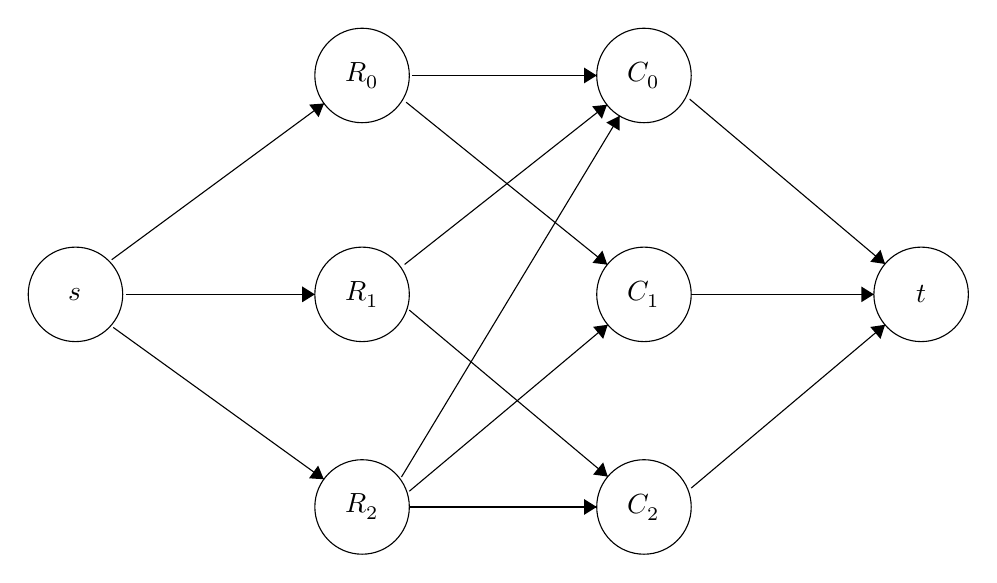
\begin{tikzpicture}[scale=0.2]
\tikzstyle{every node}+=[inner sep=0pt]
\draw [black] (12.2,-28.8) circle (3);
\draw (12.2,-28.8) node {$s$};
\draw [black] (65.9,-28.8) circle (3);
\draw (65.9,-28.8) node {$t$};
\draw [black] (30.4,-42.3) circle (3);
\draw (30.4,-42.3) node {$R_2$};
\draw [black] (48.3,-28.8) circle (3);
\draw (48.3,-28.8) node {$C_1$};
\draw [black] (48.3,-14.9) circle (3);
\draw (48.3,-14.9) node {$C_0$};
\draw [black] (48.3,-42.3) circle (3);
\draw (48.3,-42.3) node {$C_2$};
\draw [black] (30.4,-28.8) circle (3);
\draw (30.4,-28.8) node {$R_1$};
\draw [black] (30.4,-14.9) circle (3);
\draw (30.4,-14.9) node {$R_0$};
\draw [black] (51.3,-41.1) -- (63.61,-30.73);
\fill [black] (63.61,-30.73) -- (62.67,-30.87) -- (63.32,-31.63);
\draw [black] (51.3,-28.8) -- (62.9,-28.8);
\fill [black] (62.9,-28.8) -- (62.1,-28.3) -- (62.1,-29.3);
\draw [black] (15.4,-28.8) -- (27.4,-28.8);
\fill [black] (27.4,-28.8) -- (26.6,-28.3) -- (26.6,-29.3);
\draw [black] (14.5,-26.6) -- (27.98,-16.68);
\fill [black] (27.98,-16.68) -- (27.04,-16.75) -- (27.64,-17.55);
\draw [black] (14.6,-30.9) -- (27.97,-40.54);
\fill [black] (27.97,-40.54) -- (27.61,-39.67) -- (27.03,-40.48);
\draw [black] (51.2,-16.4) -- (63.61,-26.87);
\fill [black] (63.61,-26.87) -- (63.32,-25.97) -- (62.67,-26.73);
\draw [black] (33.6,-14.9) -- (45.3,-14.9);
\fill [black] (45.3,-14.9) -- (44.5,-14.4) -- (44.5,-15.4);
\draw [black] (33.2,-16.6) -- (45.97,-26.91);
\fill [black] (45.97,-26.91) -- (45.66,-26.02) -- (45.03,-26.8);
\draw [black] (33.4,-29.8) -- (46,-40.37);
\fill [black] (46,-40.37) -- (45.71,-39.47) -- (45.07,-40.24);
\draw [black] (33.4,-42.3) -- (45.3,-42.3);
\fill [black] (45.3,-42.3) -- (44.5,-41.8) -- (44.5,-42.8);
\draw [black] (33.4,-41.3) -- (46,-30.73);
\fill [black] (46,-30.73) -- (45.07,-30.86) -- (45.71,-31.63);
\draw [black] (32.9,-40.4) -- (46.75,-17.47);
\fill [black] (46.75,-17.47) -- (45.91,-17.89) -- (46.76,-18.41);
\draw [black] (33.1,-26.9) -- (45.95,-16.76);
\fill [black] (45.95,-16.76) -- (45.01,-16.86) -- (45.63,-17.65);
\end{tikzpicture}

\textbf{\\Edges from $S$ to $R_i$}: weight = $p$\\
\textbf{Edges from $R_i$ to $C_i$}: weight = $1$\\
\textbf{Edges from $C_i$ to $t$}: weight = $p$
\end{center}}

Now, all that remains is running the Ford-Fulkerson or Edmond-Karp algorithm to determine maxflow.

\mybox{\centering If \textbf{MAXFLOW = n $\cdot$ p $\implies$ $\exists$ solution.}}

The above is true, because each column, $C_i$ must supply $p$ flow for a solution to exist, and there are $n$ columns $\implies$ $n$ $C_i$ nodes. \\

\textbf{Runtime analysis}:
\mybox{There are $2n$ nodes and at most $n^2$ vertices, so using E-K we would expect:
$$\sim O(n^4)$$

Using F-F, we would expect:
$$\sim O(n^2 \cdot n \cdot p) = O(n^3p)$$
}

The setup outlined above is predicated on knowledge of the correct $p$ which can be easily found via an $O(n^2)$ algorithm wherein two size-$n$ arrays keep track of totals of plots with soil per row and column (iterative process updated through an entire traversal of $n \times n$ matrix).  Locating the global minimum in the two size-$n$ arrays will provide an \textbf{upper-bound} for $p$ (ideally reachable).  It should be noted that a loose upper-bound for $p$ is $n$.\\

Because this one-time $p$-finding-process is much smaller than the run of E-K or F-F, it is omitted from the asymptotic analysis; however, now knowing an upper bound for $p$ we can revise our runtime for F-F: $\implies O(n^4)$.\\

Finally, it should also be noted that the process described above must be run for each value of $p$ we try up to the upper bound of $p$ (note @759 on Piazza mentions that if $\exists$ a satisfiable $p$ such that maxflow = $np$, then $p-1$ also has a satisfiable maxflow = $(n)(p-1)$, so we would run E-K or F-F $p$ times before guaranteeing success or no-success). \\

Revised runtime analysis:
\mybox{
Running E-K or F-F $p$ times, given $p \sim O(n)$:
$$\mathbf{\sim O(n^5)}$$ 
}
Supposedly, in speaking to Jaylen W., this runtime can be reduced as well via the note @759 on Piazza wherein we can \enquote{save} our residual graphs each run of F-F [if $\exists$ a satisfiable $p$ such that maxflow = $np$, then $p-1$ also has a satisfiable maxflow = $(n)(p-1)$]; thereby, far reducing the majority of our runtime.  I am not sure how to prove correctness for this extension, so I will just leave it as a note.

\newpage
\subsection{Failure}
It is worth noting that I had believed I could solve this problem in $\sim O(n^2)$ runtime via a greedy algorithm---after all, who doesn't love a simple, easy to implement greedy alg?  Unfortunately, it seems, this \enquote{Sudoku} type problem (as my friend Benny put it) is not so easy...that's why Sudoku is challenging, I guess.  Here's some of my failed code with a failed output:

\begin{figure}[h!]
    \centering
    \includegraphics[width=0.2\textwidth]{P3 Figs/Q3_greedyFails.png}
    \caption{Solvable if planted palm trees on anti-diagonal}
    \label{fig:greedyFails}
\end{figure}
\FloatBarrier


\begin{minted}[fontsize=\footnotesize]{c++}
void fillTracker(vector< vector<int> > &land, vector< vector<int> > &tracker, 
int dimension) {
    for (int i = 0; i < dimension; i++) {
        for (int j = 0; j < dimension; j++) {
            if (land[i][j] == 1) {
                tracker[0][i]++; // increment row count
                tracker[1][j]++; // increment col count
            }
        }
    }
}

int findmin(vector< vector<int> > &tracker, int dimension) {
    int globalmin = tracker[0][0];

    for (int i = 0; i < 2; i++) {
        for (int j = 0; j < dimension; j++) {
            globalmin = (tracker[i][j] < globalmin) ? tracker[i][j] : globalmin;
        }
    }
    return globalmin;
}

void setmin(vector< vector<int> > &tracker, int dimension, int p){
    for (int i = 0; i < 2; i++) {
        for (int j = 0; j < dimension; j++) {
            tracker[i][j] = p;
        }
    }
}


void planters(vector< vector<int> > &land, vector< vector<int> > &tracker,
int dimension, int p) {
    for (int i = 0; i < dimension; i++) {
        for (int j = 0; j < dimension; j++) {
            if ((tracker[0][i] > 0) && (tracker[0][j] > 0) && (land[i][j] == 1)){
                land[i][j] = 1;
                tracker[0][i]--; // decrement row count
                tracker[1][j]--; // decrement col count
            }
            else {
                land[i][j] = 0;
            }
        }
    }
}

// RANDOM MATRIX GENERATOR
void randm(vector< vector<int> > &land, int dimension) {
    random_device seed;
    static mt19937 generator(seed());
    uniform_int_distribution<int> dis(0, 1);
    for (int i = 0; i < dimension; i++) {
        for (int j = 0; j < dimension; j++) {
            land[i][j] = dis(generator);
        }
    }
}

int main(int argc,char* argv[])
{
    int dimension = 4;
    if (argc == 2){
        dimension = atoi(argv[1]);
    }

    vector<int> dimensionlong(dimension, 0);
    vector<vector<int> >land(dimension, dimensionlong), tracker(2, dimensionlong);
    randm(land, dimension);
    fillTracker(land, tracker, dimension);
    int p = findmin(tracker, dimension);
    setmin(tracker, dimension, p);
    planters(land, tracker, dimension, p);
    return 0;
}
\end{minted}





\newpage


\section{Reduction to Linear Programming}
%%%%%%%%%%%%%%%%%%
%   Question #4  %
%%%%%%%%%%%%%%%%%%
\subsection{Half 'n Half} \label{section:4a}
Let's first begin by defining variables to represent our maximization goal as well as explicit and inherent constraints, taking our network as a directed graph.\\

It is not specified, so I will take we have a source (or sources) $s_i$ whose supply is unconstrained.  We have a destination $t$ whose \enquote{in-flow} is the sum of all out-flows of nodes with directed edges to $t$.

\mybox{
$$\textbf{max} \sum_{\forall (v,t) \in E} f_{(v_i,t)}$$

$$\frac{1}{2} \sum_{\forall (u,v) \in E}f_{(u,v)} = \sum_{\forall (v,w) \in E}f_{(v,w)}$$
}

Finally, we have to constrain all flows to capacities, $k$, along edges!
\mybox{
$$0 \leq f_{(u,v)} \leq k_{(u,v)}\ \ \ \ \ \forall (u,v) \in E$$
}
This reduction to LP is synonymous, as we equivalently indicate that half the flow into a vertex is lost, and we maximize for the final flow into $t$.





\subsection{Always low prices}
Now, we add an additional goal.  Given a found max-flow found in Section \ref{section:4a}, we seek to minimize cost, $c$.\\

Using the linear program from the previous section, we can assign our \textbf{MAX FLOW = F}.  Now, we must minimize cost while ensuring that our flow reaching $t$ sums to the previously found $F$.

\mybox{
$$\textbf{min}\sum_{\forall (u,v) \in E}c_{(u,v)}f_{(u,v)}$$

$$\sum_{\forall (v,t) \in E} f_{(v_i,t)} = F$$

}

Finally, we have to constrain all costs to be non-negative!
\mybox{
$$0 \leq c_{(u,v)}\ \ \ \ \ \ \ \ \forall (u,v) \in E$$
}
This reduction to LP is synonymous with the problem statement, as we equivalently constrain our flow to node $t$ to be the previously found maximum flow and merely minimize for cost given that we're meeting the aforementioned constraint.




\newpage



\section{Two-Player Game}
%%%%%%%%%%%%%%%%%%
%   Question #5  %
%%%%%%%%%%%%%%%%%%
\subsection{Row Player}
For the row player, we wish to maximize the payout $\coloneq Z$.  We can write the following constraints given probabilities, $r_i$, corresponding to the row player's selection of each row.
\begin{align*}
    Z & \leq 3r_0 + 6r_1 - 3r_2 - 7r_3\\
    Z & \leq r_0 - 2r_1 - 2r_2 + 4r_3\\
    Z & \leq 0r_0 - 2r_1 + 3r_2 - 5r_3\\
    Z & \leq -4r_0 + 0r_1 - 3r_2 + 7r_3
\end{align*}

Re-arranging, we have our full constraints for the row player as follows:
\myalignbox{
\begin{align}
    Z - 3r_0 - 6r_1 + 3r_2 + 7r_3 & \leq 0\\
    Z - r_0 + 2r_1 + 2r_2 - 4r_3 & \leq 0\\
    Z + 2r_1 - 3r_2 + 5r_3& \leq 0\\
    Z + 4r_0 + 3r_2 - 7r_3 & \leq 0 \\
    r_0 + r_1 + r_2 + r_3 &= 1\\
    r_0,\ r_1,\ r_2,\ r_3 & \geq 0 \\
    Z \textbf{ unrestricted}
\end{align}
}

\subsection{Column Player}
For the column player, we wish to minimize the payout $\coloneq W$.  We can write the following constraints given probabilities, $c_i$, corresponding to the column player's selection of each row.
\begin{align*}
    W & \geq 3c_0 + c_1 + 0c_2 - 4c_3\\
    W & \geq 6c_0 - 2c_1 - 2c_2 + 0c_3\\
    W & \geq -3c_0 - 2c_1 + 3c_2 - 3c_3\\
    W & \geq -7c_0 + 4c_1 - 5c_2 + 7c_3
\end{align*}

Re-arranging, we have our full constraints for the row player as follows:
\myalignbox{
\begin{align}
    W -3c_0 - c_1 + 4c_3 & \geq 0\\
    W -6c_0 + 2c_1 + 2c_2 & \geq 0\\
    W +3c_0 + 2c_1 - 3c_2 + 3c_3 & \geq 0\\
    W +7c_0 - 4c_1 + 5c_2 - 7c_3 & \geq 0\\
    c_0 + c_1 + c_2 + c_3 &= 1\\
    c_0,\ c_1,\ c_2,\ c_3 & \geq 0 \\
    W \textbf{ unrestricted}
\end{align}
}

\subsection{Solved}
Using \verb|online-optimizer.appspot.com| (i.e., the first link on Google), I optimized for both the Row and Column Players.

\subsubsection{Row Player}
The following probabilities should be used for the Row Player's strategy:
\myalignbox{
\begin{align*}
    r_0 &= 0.1509434\\
    r_1 &= 0.2761578\\
    r_2 &= 0.3790738\\
    r_3 &= 0.193825
\end{align*}}

\subsubsection{Column Player}
The following probabilities should be used for the Column Player's strategy:
\myalignbox{
\begin{align*}
    c_0 &= 0.1389365\\
    c_1 &= 0.2075472\\
    c_2 &= 0.4013722\\
    c_3 &= 0.2521441
\end{align*}}

\subsection{Value}
\mybox{\centering
The value of the game is $\mathbf{\approx -0.38}$ payout to the \textbf{row} player, \\
which represents $\mathbf{\approx 0.38}$ winnings for the \textbf{column} player. \\
The column player should thus pay the row player that amount to create a fair starting point.}








\newpage

\end{document}
